\chapter{Úvod}
Tato práce se zabývá principy jednotného přihlášení SSO. Obsahuje základní informace o různých řešeních a dále se blíže zabývá standardem SAML a jeho implementací v podobě Shibbolethu. Tato práce také obsahuje návody jak shibboleth zprovoznit, napojit na různé poskytovatele identity a následně využít při psaní aplikací.
TODO:
\section{terminologie}
\subsection{autentizace}
proces ověření identity subjektu. Většinou následuje autorizace.\cite{Authorization}
\subsection{autorizace}
proces pro specifikování přístupových práv ke zdrojům.\cite{Autentizace}

\chapter{SSO}
\label{sso}
SSO (Single Sign-On) je mechanizmus pro jednotné přihlášení. Umožňuje uživateli se přihlásit na jednom místě a následně využívat toto přihlášení pro přístup k více nezávislým aplikacím. \cite{SSO}

\section{SAML}

SAML\cite{SAMLofficialSite}\cite{WhatIsSaml} (Security Assertion Markup Language) je otevřený standard umožňující výměnu autentizačních a autorizačních dat mezi více nezávislými subjekty. Využívá k tomu protokol XML. 

SAML definuje tři role. Uživatel, identity provider (zkráceně idp) a service provider (zkráceně sp). 

Identity provider(idp) se stará o autentizaci uživatele a následné poskytnutí dat service provideru(sp).

Service provider se stará o autorizaci uživatele ke svým zdrojům na základě informací poskytnutých od service provideru.

\subsection{autentizace}



\section{OIDC}

OIDC (OpenID Connect) je otevřený standard umožňující výměnu autentizačních a autorizačních dat mezi více nezávislými subjekty. Je postavený nad protokolem OAuth 2.0.\cite{OIDC}

\subsection{authentifikace}

\section{SAML x OIDC}

SAML je starší z těchto dvou protokolů a využívá k přenosu dat XML. OIDC je novější a využívá k přenosu dat JSON. 
SAML je momentálně rozšířenější i když OIDC nabírá na popularitě díky jednodušší implementaci a použítí JSONu ke komunikaci.\cite{SAMLxOIDC}
Princip přihlašování je až na různé názvosloví podobný.

\section{Shibboleth}

Shibboleth je implementace SAML standardu. Jeho hlavní součástí jsou dvě aplikace. Identity provider, který se stará o autentizaci. Service provider, který se stará o autorizaci po úspěšném přihlášení přes identity providera. \cite{shibbolethWiki}

\subsection{identity provider}

Identity provider se stará o autentizaci uživatelů. Identity provider po autentizaci uživatele předá service provideru informaci o úspěšné authentizaci společně s různými atributy.

\subsection{service provider}

Service provider se stará o autorizaci přístupu k různým službám, které poskytuje, na základě informací poskytnutých od identity provideru.

\subsection{postup přihlášení za pomocí idp}

Rozlišují se dvě možnosti přihlášení. Přihlášení vyvolané na straně identity provideru a přihlášení vyvolané na straně service provideru.


Pokud bylo přihlášení vyvolané na straně service provideru, tak je uživatel přesměrován na idp, kde bude identity providerem vyzván k autentizaci.
Po úspěšné autentizaci identity provider předá informaci o úspěšné autentizaci společně s různými atributy, na kterých se předem domluvily, service provideru společně s přesměrováním uživatele na původní stránku.
Tyto informace service provider využije k autorizaci různých svých částí.\cite{SAMLxOIDC}
\begin{figure}[bp]
	\centering
    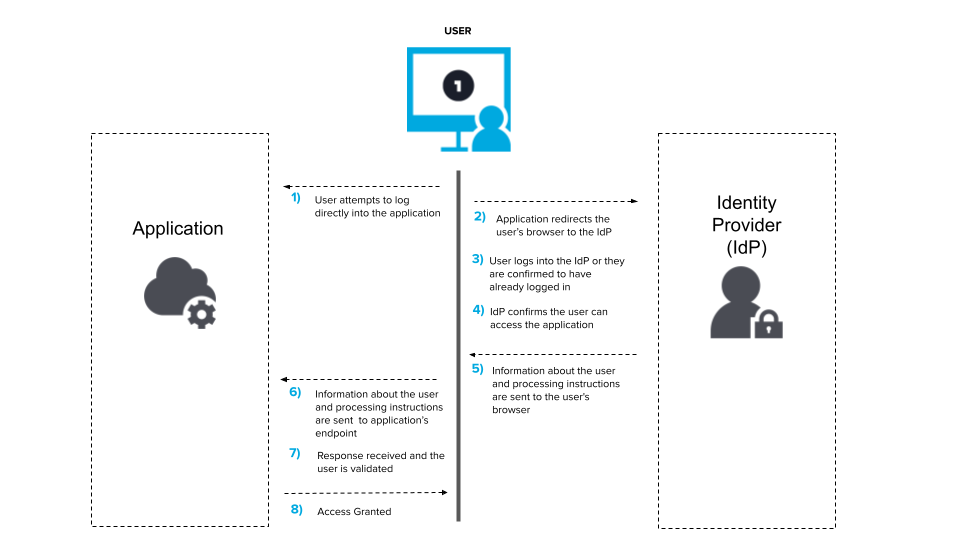
\includegraphics[width=1.2\textwidth]{obrazky-figures/saml-sp.png}
	\caption{Ukázka přihlášení vyvolané sp\cite{SAMLxOIDC}}
	\label{saml-flow}
\end{figure}

Pokud bylo přihlášení vyvolané na straně identity provideru, tak je uživatel rovnou přesměrován na service provideru s informaci o úspěšné autentizaci společně s různými atributy, na kterých se předem domluvily.
Tyto informace service provider využije k autorizaci různých svých částí.\cite{SAMLxOIDC}

\begin{figure}[bp]
	\centering
    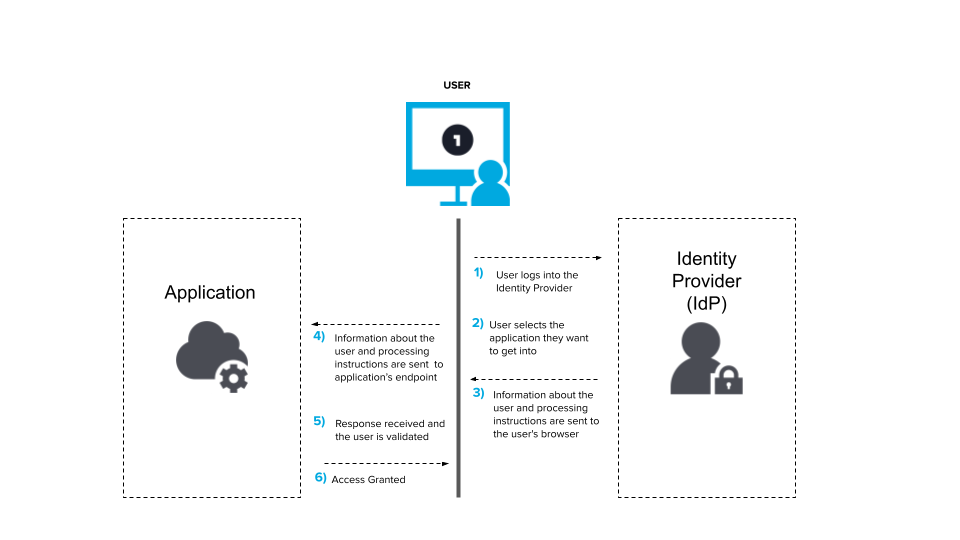
\includegraphics[width=1.2\textwidth]{obrazky-figures/saml-idp.png}
	\caption{Ukázka přihlášení vyvolané idp\cite{SAMLxOIDC}}
	\label{saml-flow}
\end{figure}
\chapter{Návod}
\label{návod}

Zde je návod jak nainstalovat a nastavit Shibboleth sp, tak aby ho bylo možné propojit s idp. Jedná se převážně o aktualizaci tohoto návodu\cite{shibbolethSpInstallation}, v kombinaci s informacemi na oficiální wiki shibbolethu\cite{shibbolethWikiSP}

\section{Instalace sp}

Nejdříve je třeba nainstalovat web server. Tento návod využívá Apache2
\begin{lstlisting}[language=Bash]
    sudo apt-get update
    sudo apt-get install apache2
\end{lstlisting}

Dále je třeba vygenerovat certifikáty pro Apache2. Pro jednoduchost se vygenerují self-signed certifikáty.
\begin{lstlisting}[language=Bash]
    sudo a2enmod ssl
    sudo a2ensite default-ssl.conf
    sudo mkdir /etc/apache2/ssl
    sudo openssl req -x509 -nodes -days 365 -newkey rsa:2048 \
    -keyout /etc/apache2/ssl/apache.key -out /etc/apache2/ssl/apache.crt
\end{lstlisting}

Shibboleth potřebuje vygenerovat certifikát ke komunikaci s idp. Localhost je třeba nahradit ipadresou serveru na kterém sp poběží.
\begin{lstlisting}[language=Bash]
    sudo shib-keygen -h localhost
    openssl x509 -text -noout -in /etc/shibboleth/sp-cert.pem
\end{lstlisting}

Nastavení shibolethu se nachází /etc/shibboleth/shibboleth2.xml .

\begin{lstlisting}[language=Bash]
   sudo vim /etc/shibboleth/shibboleth2.xml
\end{lstlisting}

Zde je potřeba nastavit následující hodnoty. V <ApplicationDefaults> je potřeba nastavit entityID. EntityID by mělo být jedinečné. Většinou se používá doména aplikace ke které se bude přistupovat přes Shibboleth. Například: http://vasedomena/shibboleth . Není to ale nutné pro fungování Shibbolethu.

Pro povolení SSL, je třeba nastavit v <Sessions>  handlerSSL na true a cookieProps na https.

Pod <SSO> se přidá EntityID idp, který se bude používat.

Na konec souboru se přidá informace kde se nachází metadata idp.
\begin{lstlisting}[language=Bash]
 <MetadataProvider type="XML" validate="true"
                url="https://samltest.id/saml/idp"/>
\end{lstlisting}

pro jednoduchost se použije jeden klíč pro podpis i pro šifrování.

Toho se docílí změnou těchto řádků:
\begin{lstlisting}[language=Bash]
<CredentialResolver type="File" use="signing"
            key="sp-signing-key.pem" certificate="sp-cert.pem"/>
        <CredentialResolver type="File" use="encryption"
            key="sp-encrypt-key.pem" certificate="sp-cert.pem"/>
\end{lstlisting}

na tyto:
\begin{lstlisting}[language=Bash]
<CredentialResolver type="File"
            key="sp-key.pem" certificate="sp-cert.pem"/>
\end{lstlisting}

následně je třeba restartovat shibboleth
\begin{lstlisting}[language=Bash]
sudo service shibd restart
\end{lstlisting}

Pokud vše funguje, tak na následující adrese by měl být vidět text: "A valid session was not found."
\begin{lstlisting}[language=Bash]
https://vasedomena/Shibboleth.sso/Session
\end{lstlisting}

\section{Propojení s idp}

Zde je uvedeno pár návodů pro propojení sp s různými idp.

\subsection{SAML test}
SAML test je testovací stránka pro debugování SAML aplikací. Většina idp bude mít stejný postup propojení jako SAML test.



Na tuto stránku je třeba nahrát metadata z sp 
\url{https://samltest.id/upload.php}  . Tyto metadata se dají získat na následující cestě na doméně kde je hostován SP \url{https://vasedomena/Shibboleth.sso/Session }

dále je potřeba v nastavení shibbolethu (/etc/shibboleth/shibboleth2.xml) přidat cestu k metadatům idp.
\begin{lstlisting}[language=Bash]
 <MetadataProvider type="XML"
                url="https://samltest.id/saml/idp"/>
\end{lstlisting}

Následně když se zajde na tuto stránku \url{https://samltest.id/start-sp-test/}, tak po vyplnění entityID se dá přihlásit do SP, přes samltest idp.

Po přihlášení by mělo být vidět na následující cestě na doméně kde je hostován SP informace o aktivním sessionu \url{http://vasedomena/Shibboleth.sso/Session} 



\subsection{Azure}

Tato sekce je inspirována tímto návodem\cite{AzureTutorial}


Pro propojení s Azure IDP je potřeba udělat následující kroky
\begin{itemize}
    \item v Azure portalu u Azure services je třeba kliknout na Azure Active Directory
    \item vlevo ve sloupci pod manage otevřít Enterprise applications
    \item kliknout na New application
    \item kliknout na Create your own application
    \item tlačítkem Create potvrdit vytvoření aplikace
    \item v aplikaci vlevo pod položkou Single sign-on se vybere SAML a dále jsou potřeba nastavit následující
    \item Basic SAML Configuration
    \begin{itemize}
        \item Identifier je třeba nastavit na entityID SP
        \item Reply URL je třeba nastavit na \url{https://vasedomena/Shibboleth.sso/SAML2/POST}
    \end{itemize}
    \item \mbox{ Attributes \& Claims} \linebreak
    Protože Azure využívá pro NameID SAML identifier místo SAML atributu, tak je potřeba pro NameID nastavit Name identifier format na Unspecified.
    Dále stačí vybrat, jaký atribut se bude používat pro identifikaci uživatele.
    
    Následně je ještě potřeba v nastavení SP v souboru attribute-map.xml (/etc/shibboleth/attribute-map.xml) přidat následující řadky:
    
    \begin{lstlisting}[language=XML]
   <Attribute name="urn:oasis:names:tc:SAML:1.1:nameid-format:unspecified"
   id="NameID">
        <AttributeDecoder xsi:type="NameIDAttributeDecoder" 
        formatter="$Name" defaultQualifiers="true"/>
   </Attribute>
\end{lstlisting}
které řeknou Shibboleth jak interpretovat NameID. NameID bude uloženo v proměnné NameID.

Jakékoli další atributy, které je potřeba předávat SP, se dají nastavit na této stránce podobným způsobem. Name format se nechá na Omitted, jinak zbytek nastavení je dle potřeb aplikace. Následně je potřeba do attribute-map.xml přidat informaci jak se mají jednotlivé atributy zpracovat.
   \begin{lstlisting}[language=XML]
     <Attribute name="Namespace/Name"
    nameFormat="urn:oasis:names:tc:SAML:2.0:attrname-format:unspecified"
    id="role1" />
    \end{lstlisting}
Namespace se nahradí za namespace atributu. Name se nahradí za název atributu. Pokud bylo potřeba měnit Name Format, tak je ho potřeba změnit i zde.\cite{AddAttribute}
    


    \item Dále je třeba nahrát pomocí tlačítka vlevo nahoře "Upload metadata file" metadata SP. Tyto metadata najdete na této cestě u vašeho SP \url{http://vasedomena/Shibboleth.sso/Metadata}

\end{itemize}

Po nastavení se dá aplikace otestovat tlačítkem Test. Aplikace by vás měla přesměrovat na doménu vaší aplikace a následně na následující adrese \url{https://vasedomena/Shibboleth.sso/Session} by měla být vidět aktivní session a názvy atributů, které IDP předal SP.

\section{používání v Apache}

Pro využití shibolethu v Apache stačí uvést do .htaccess co je vyžadováno za oprávnění od uživatele. Více informací o sytaxi je k nalezení v dokumentaci\cite{SPApache}\cite{SPhtaccess} \linebreak

příklad .htaccess pro přístup uživatele testuser@gmail.com:

 \begin{lstlisting}[language=XML]
    AuthType shibboleth
ShibRequestSetting requireSession true
<RequireAll>
  require shibboleth
  require shib-user testuser@gmail.com
</RequireAll>
    \end{lstlisting}


\section{Discovery service}
Pro používání více než jednoho idp je potřeba nastavit discovery service, kde si může uživatel vybrat kterého chce použít identity providera. Pro jednoduché řešení stačí statická webová stránka s přesměrováními na různé identity providery, pro řešení obsahující desítky idp je lepší využít discovery service od Shibbolethu. Zde hodně záleží na konkrétní aplikaci. Různé možnosti implementace jsou popsané v dokumentaci \cite{IdPDiscovery}.

\subsection{Embedded Discovery Service}
Je jednoduchá applikace od shibboleth napsaná v javascriptu. 

\subsection{Embedded Discovery Service - návod}
Tato sekce byla inspirována následujícím návodem TODO .
instalace EDS
\begin{lstlisting}[language=Bash]
  sudo su -

cd /usr/local/src

wget https://shibboleth.net/downloads/embedded-discovery-service/latest/shibboleth-embedded-ds-1.2.2.tar.gz -O shibboleth-eds.tar.gz

tar xzf shibboleth-eds.tar.gz

cd shibboleth-embedded-ds-1.2.2

apt install make

make install
\end{lstlisting}

povolení webové stránky EDS

\begin{lstlisting}[language=Bash]
mv /etc/shibboleth-ds/shibboleth-ds.conf /etc/apache2/conf-available/shibboleth-ds.conf

a2enconf shibboleth-ds.conf

systemctl restart apache2.service
\end{lstlisting}

V Shibboleth SP nastavení (/etc/shibboleth/shibboleth2.xml), je potřeba udělat následující:
1. SSO přepsat následovně:

\begin{lstlisting}[language=Bash]
<SSO discoveryProtocol="SAMLDS" 
     discoveryURL="https://###YOUR.SP.FQDN###/shibboleth-ds/index.html">
   SAML2 SAML1
</SSO>
\end{lstlisting}

odkomentovat DiscoveryFeed handler a SessionInitiator handler

\begin{lstlisting}[language=Bash]
<Handler type="DiscoveryFeed" Location="/DiscoFeed"/>
 <Handler type="SessionInitiator" Location="/Login"/>
\end{lstlisting}

následně je třeba restartovat shibd a apache2 .

\begin{lstlisting}[language=Bash]
systemctl restart shibd.service
systemctl restart apache2.service
\end{lstlisting}

Dále je potřeba nastavit whitelist návratových adress v souboru idpselect_config.js, který se nachází v nastavení EDS (/etc/shibboleth-ds/idpselect_config.js)

v položce this.returnWhiteList je třeba změnit url aby odpovídala vašemu SP. 

\begin{lstlisting}[language=Bash]
this.returnWhiteList = [ "^https:\/\/vasedomena\.com\/Shibboleth\.sso\/Login.*$" , "^https:\/\/vasedomena\.com\/Shibboleth\.sso\/Login.*$" ];
\end{lstlisting}

Teď když zkusíte na vaši stránce zajít na nějaký zdroj chráněný pomocí Shibboleth, tak by vás to mělo přesměrovat na stránku podobnou té na následujícím obrázku:
Zde se dá jednoduše vybrat idp, na jehož přihlašovací obrazovku vás to následně přesměruje.

\chapter{config}
Popis důležitých částí nastavení, které jsou nutné k správnému fungování shibboleth sp. Detailní informace jsou k nalezení na webu\cite{SPconfig}. 

\section{shibboleth2.xml}
Hlavní config soubor shibbolethu. Nachází se na cestě /etc/shibboleth/shibboleth2.xml .

\subsection{ApplicationDefaults}
\begin{lstlisting}[language=xml]
<ApplicationDefaults entityID="https://vasedomena/shibboleth"
        REMOTE_USER="NameID"
        cipherSuites="DEFAULT:!EXP:!LOW:!aNULL:!eNULL:!DES:!IDEA:
        !SEED:!RC4:!3DES:!kRSA:!SSLv2:!SSLv3:!TLSv1:!TLSv1.1">
\end{lstlisting}
\begin{itemize}
    \item entityID \linebreak
    Název SP. Musí být unikátní v rámci federace identit. Je zvykem využít doménu sp.  
    \item REMOTE\_USER \linebreak
    Zde patří názvy atributů, kterými se budou od sebe odlišovat různí uživatelé. 
    Tento atribut bude následně k dispozici z proměnné REMOTE\_USER.
\end{itemize}
\subsection{MetadataProvider}
Definuje kde se nachází metadata identity provideru. Pro většinu aplikací by mělo stačit jedno z následujících nastavení. Více informací lze nalézt na webových stránkách\cite{MetadataProvider}.
\linebreak \linebreak
Metadata se nahrávají z url.
\begin{lstlisting}[language=Bash]
 <MetadataProvider type="XML" validate="true"
                url="https://samltest.id/saml/idp"/>
\end{lstlisting}
Metadata se nahrávají ze souboru.
\begin{lstlisting}[language=Bash]
 <MetadataProvider type="XML" path="/path/to/the/metadata.xml"/>
\end{lstlisting}


\section{attribute-map.xml}
TODO: https://shibboleth.atlassian.net/wiki/spaces/SP3/pages/2070414225/XMLAttributeExtractorExamples
Obsahuje informace o mapování atributů přijatých od identity provideru na proměnné service provideru. Soubor obsahuje nějaké základní mapování, ale pro většinu aplikací bude nutné tento soubor upravit.

Následuje příklad přidání jednoduchého atributu, kde jméno atributu přijatého od idp je FavoriteFruit a favFruit je jméno používané v proměnných sp\cite{AddAttribute}.
 \begin{lstlisting}[language=XML]
     <Attribute name="FavoriteFruit"
    nameFormat="urn:oasis:names:tc:SAML:2.0:attrname-format:basic"
    id="favFruit" />
    \end{lstlisting}
    
Toto nastavení by mělo být dostačující pro většinu aplikací. Více informací lze nalézt na webových stránkách\cite{AddAttribute}.

\chapter{Závěr}
TODO:
\label{zaver}






%===============================================================================
